\documentclass[12pt, a4paper, openany, twoside]{book}
\usepackage[left=1in,right=1in,bottom=1in,top=1in]{geometry}
\usepackage[most]{tcolorbox}
\usepackage{amssymb}
\usepackage{amsthm}
\usepackage{lastpage}
\usepackage{fancyhdr}
\usepackage{amsfonts}
\usepackage{amsmath, amssymb}
\usepackage{graphicx}
\usepackage[font=small,labelfont=bf]{caption}
\usepackage{epstopdf}
\usepackage{xcolor}
\usepackage{amsthm}
\usepackage{float}
\usepackage{pgfplots}
\usepackage{listings}
\usepackage{longtable}
\usepackage{mathrsfs}
\usepackage{mathtools}
\usepackage{amssymb}
\usepackage{enumitem}
\usepackage{array}
\usepackage{tikz-cd}
\usepackage{extpfeil}
\usepackage{etoolbox}
\usepackage[pdfpagelabels,hyperindex,colorlinks=true, linkcolor=blue, citecolor=red, urlcolor=magenta, filecolor=cyan]{hyperref}


\hypersetup{
pdftitle={Lebesgue Integral Theory},
pdfauthor={Jaeho Shin},
}

\newcommand{\overbar}[1]{\mkern 1.5mu\overline{\mkern-1.5mu#1\mkern-1.5mu}\mkern 1.5mu}
\DeclareRobustCommand{\stirling}{\genfrac\{\}{0pt}{}}
\newtheorem{thm}{Theorem}[section]
\newtheorem{cor}[thm]{Corollary}
\newtheorem{prop}[thm]{Proposition}
\newtheorem{lem}[thm]{Lemma}
\newtheorem{conj}[thm]{Conjecture}
\newtheorem{quest}[thm]{Question}
\newtheorem{ppty}[thm]{Property}
\newtheorem{ppties}[thm]{Properties}
\newtheorem{axiom}[thm]{Axiom}
\newtheorem{claim}[thm]{Claim}
\newtheorem{prob}[thm]{Problem}


\theoremstyle{definition}
\newtheorem{defn}[thm]{Definition}
\newtheorem{defns}[thm]{Definitions}
\newtheorem{con}[thm]{Construction}
\newtheorem{exmp}[thm]{Example}
\newtheorem{exmps}[thm]{Examples}
\newtheorem{notn}[thm]{Notation}
\newtheorem{notns}[thm]{Notations}
\newtheorem{addm}[thm]{Addendum}
\newtheorem{exer}[thm]{Exercise}
\newtheorem{limit}[thm]{Limitation}


\theoremstyle{remark}
\newtheorem{rem}[thm]{Remark}
\newtheorem{rems}[thm]{Remarks}
\newtheorem{warn}[thm]{Warning}
\newtheorem{sch}[thm]{Scholium}


    % newcommand bb
    \newcommand{\BA}{{\mathbb {A}}} \newcommand{\BB}{{\mathbb {B}}}
    \newcommand{\BC}{{\mathbb {C}}} \newcommand{\BD}{{\mathbb {D}}}
    \newcommand{\BE}{{\mathbb {E}}} \newcommand{\BF}{{\mathbb {F}}}
    \newcommand{\BG}{{\mathbb {G}}} \newcommand{\BH}{{\mathbb {H}}}
    \newcommand{\BI}{{\mathbb {I}}} \newcommand{\BJ}{{\mathbb {J}}}
    \newcommand{\BK}{{\mathbb {U}}} \newcommand{\BL}{{\mathbb {L}}}
    \newcommand{\BM}{{\mathbb {M}}} \newcommand{\BN}{{\mathbb {N}}}
    \newcommand{\BO}{{\mathbb {O}}} \newcommand{\BP}{{\mathbb {P}}}
    \newcommand{\BQ}{{\mathbb {Q}}} \newcommand{\BR}{{\mathbb {R}}}
    \newcommand{\BS}{{\mathbb {S}}} \newcommand{\BT}{{\mathbb {T}}}
    \newcommand{\BU}{{\mathbb {U}}} \newcommand{\BV}{{\mathbb {V}}}
    \newcommand{\BW}{{\mathbb {W}}} \newcommand{\BX}{{\mathbb {X}}}
    \newcommand{\BY}{{\mathbb {Y}}} \newcommand{\BZ}{{\mathbb {Z}}}

    % newcommand  scr
    \newcommand{\sA}{{\mathscr {A}}} \newcommand{\sB}{{\mathscr {B}}}
    \newcommand{\sC}{{\mathscr {C}}} \newcommand{\sD}{{\mathscr {D}}}
    \newcommand{\sE}{{\mathscr {E}}} \newcommand{\sF}{{\mathscr {F}}}
    \newcommand{\sG}{{\mathscr {G}}} \newcommand{\sH}{{\mathscr {H}}}
    \newcommand{\sI}{{\mathscr {I}}} \newcommand{\sJ}{{\mathscr {J}}}
    \newcommand{\sK}{{\mathscr {K}}} \newcommand{\sL}{{\mathscr {L}}}
    \newcommand{\sN}{{\mathscr {N}}} \newcommand{\sM}{{\mathscr {M}}}
    \newcommand{\sO}{{\mathscr {O}}} \newcommand{\sP}{{\mathscr {P}}}
    \newcommand{\sQ}{{\mathscr {Q}}} \newcommand{\sR}{{\mathscr {R}}}
    \newcommand{\sS}{{\mathscr {S}}} \newcommand{\sT}{{\mathscr {T}}}
    \newcommand{\sU}{{\mathscr {U}}} \newcommand{\sV}{{\mathscr {V}}}
    \newcommand{\sW}{{\mathscr {W}}} \newcommand{\sX}{{\mathscr {X}}}
    \newcommand{\sY}{{\mathscr {Y}}} \newcommand{\sZ}{{\mathscr {Z}}}


    % newcommand cal
    \newcommand{\CA}{{\mathcal {A}}} \newcommand{\CB}{{\mathcal {B}}}
    \newcommand{\CC}{{\mathcal {C}}} \newcommand{\CD}{{\mathcal {D}}}
    \newcommand{\CE}{{\mathcal {E}}} \newcommand{\CF}{{\mathcal {F}}}
    \newcommand{\CG}{{\mathcal {G}}} \newcommand{\CH}{{\mathcal {H}}}
    \newcommand{\CI}{{\mathcal {I}}} \newcommand{\CJ}{{\mathcal {J}}}
    \newcommand{\CK}{{\mathcal {K}}} \newcommand{\CL}{{\mathcal {L}}}
    \newcommand{\CM}{{\mathcal {M}}} \newcommand{\CN}{{\mathcal {N}}}
    \newcommand{\CO}{{\mathcal {O}}} \newcommand{\CP}{{\mathcal {P}}}
    \newcommand{\CQ}{{\mathcal {Q}}} \newcommand{\CR}{{\mathcal {R}}}
    \newcommand{\CS}{{\mathcal {S}}} \newcommand{\CT}{{\mathcal {T}}}
    \newcommand{\CU}{{\mathcal {U}}} \newcommand{\CV}{{\mathcal {V}}}
    \newcommand{\CW}{{\mathcal {W}}} \newcommand{\CX}{{\mathcal {X}}}
    \newcommand{\CY}{{\mathcal {Y}}} \newcommand{\CZ}{{\mathcal {Z}}}

    % newcommand frak
    \newcommand{\fa}{{\mathfrak{a}}}  \newcommand{\fb}{{\mathfrak{b}}}
    \newcommand{\fc}{{\mathfrak{c}}}  \newcommand{\fd}{{\mathfrak{d}}}
    \newcommand{\fe}{{\mathfrak{e}}}  \newcommand{\ff}{{\mathfrak{f}}}
    \newcommand{\fg}{{\mathfrak{g}}}  \newcommand{\fh}{{\mathfrak{h}}}
    \newcommand{\fii}{{\mathfrak{i}}}  \newcommand{\fj}{{\mathfrak{j}}}
    \newcommand{\fk}{{\mathfrak{m}}}  \newcommand{\fl}{{\mathfrak{l}}}
    \newcommand{\fm}{{\mathfrak{m}}}  \newcommand{\fn}{{\mathfrak{n}}}
    \newcommand{\fo}{{\mathfrak{o}}}  \newcommand{\fp}{{\mathfrak{p}}}
    \newcommand{\fq}{{\mathfrak{q}}}  \newcommand{\fr}{{\mathfrak{r}}}
    \newcommand{\fs}{{\mathfrak{s}}}  \newcommand{\ft}{{\mathfrak{t}}}
    \newcommand{\fu}{{\mathfrak{u}}}  \newcommand{\fv}{{\mathfrak{v}}}
    \newcommand{\fw}{{\mathfrak{w}}}  \newcommand{\fx}{{\mathfrak{x}}}
    \newcommand{\fy}{{\mathfrak{y}}}  \newcommand{\fz}{{\mathfrak{z}}}

    \newcommand{\fA}{{\mathfrak{A}}}  \newcommand{\fB}{{\mathfrak{B}}}
    \newcommand{\fC}{{\mathfrak{C}}}  \newcommand{\fD}{{\mathfrak{D}}}
    \newcommand{\fE}{{\mathfrak{E}}}  \newcommand{\fF}{{\mathfrak{F}}}
    \newcommand{\fG}{{\mathfrak{G}}}  \newcommand{\fH}{{\mathfrak{H}}}
    \newcommand{\fI}{{\mathfrak{I}}}  \newcommand{\fJ}{{\mathfrak{J}}}
    \newcommand{\fK}{{\mathfrak{K}}}  \newcommand{\fL}{{\mathfrak{L}}}
    \newcommand{\fM}{{\mathfrak{M}}}  \newcommand{\fN}{{\mathfrak{N}}}
    \newcommand{\fO}{{\mathfrak{O}}}  \newcommand{\fP}{{\mathfrak{P}}}
    \newcommand{\fQ}{{\mathfrak{Q}}}  \newcommand{\fR}{{\mathfrak{R}}}
    \newcommand{\fS}{{\mathfrak{S}}}  \newcommand{\fT}{{\mathfrak{T}}}
    \newcommand{\fU}{{\mathfrak{U}}}  \newcommand{\fV}{{\mathfrak{V}}}
    \newcommand{\fW}{{\mathfrak{W}}}  \newcommand{\fX}{{\mathfrak{X}}}
    \newcommand{\fY}{{\mathfrak{Y}}}  \newcommand{\fZ}{{\mathfrak{Z}}}



    % newcommand :rm
    \newcommand{\RA}{{\mathrm {A}}} \newcommand{\RB}{{\mathrm {B}}}
    \newcommand{\RC}{{\mathrm {C}}} \newcommand{\RD}{{\mathrm {D}}}
    \newcommand{\RE}{{\mathrm {E}}} \newcommand{\RF}{{\mathrm {F}}}
    \newcommand{\RG}{{\mathrm {G}}} \newcommand{\RH}{{\mathrm {H}}}
    \newcommand{\RI}{{\mathrm {I}}} \newcommand{\RJ}{{\mathrm {J}}}
    \newcommand{\RK}{{\mathrm {K}}} \newcommand{\RL}{{\mathrm {L}}}
    \newcommand{\RM}{{\mathrm {M}}} \newcommand{\RN}{{\mathrm {N}}}
    \newcommand{\RO}{{\mathrm {O}}} \newcommand{\RP}{{\mathrm {P}}}
    \newcommand{\RQ}{{\mathrm {Q}}} \newcommand{\RR}{{\mathrm {R}}}
    \newcommand{\RS}{{\mathrm {S}}} \newcommand{\RT}{{\mathrm {T}}}
    \newcommand{\RU}{{\mathrm {U}}} \newcommand{\RV}{{\mathrm {V}}}
    \newcommand{\RW}{{\mathrm {W}}} \newcommand{\RX}{{\mathrm {X}}}
    \newcommand{\RY}{{\mathrm {Y}}} \newcommand{\RZ}{{\mathrm {Z}}}

    \newcommand{\Ad}{{\mathrm{Ad}}} \newcommand{\Aut}{{\mathrm{Aut}}}
    \newcommand{\Br}{{\mathrm{Br}}} \newcommand{\Ch}{{\mathrm{Ch}}}
    \newcommand{\cod}{{\mathrm{cod}}} \newcommand{\cont}{{\mathrm{cont}}}
    \newcommand{\cl}{{\mathrm{cl}}}   \newcommand{\Cl}{{\mathrm{Cl}}}
    \newcommand{\disc}{{\mathrm{disc}}}\newcommand{\Eis}{{\mathrm{Eis}}}
    \newcommand{\Div}{{\mathrm{Div}}} \renewcommand{\div}{{\mathrm{div}}}
    \newcommand{\End}{{\mathrm{End}}} \newcommand{\Frob}{{\mathrm{Frob}}}
    \newcommand{\Gal}{{\mathrm{Gal}}} \newcommand{\GL}{{\mathrm{GL}}}
    \newcommand{\Hom}{{\mathrm{Hom}}} \renewcommand{\Im}{{\mathrm{Im}}}
    \newcommand{\Ind}{{\mathrm{Ind}}} \newcommand{\ind}{{\mathrm{ind}}}
    \newcommand{\inv}{{\mathrm{inv}}}
    \newcommand{\Isom}{{\mathrm{Isom}}} \newcommand{\Jac}{{\mathrm{Jac}}}
    \newcommand{\ad}{{\mathrm{ad}}}  \newcommand{\Tr}{{\mathrm{Tr}}}
    \newcommand{\Ker}{{\mathrm{Ker}}} \newcommand{\Ros}{{\mathrm{Ros}}}
    \newcommand{\Lie}{{\mathrm{Lie}}} \newcommand{\Hol}{{\mathrm{Hol}}}

    \newcommand{\cyc}{{\mathrm{cyc}}}\newcommand{\id}{{\mathrm{id}}}
    \newcommand{\new}{{\mathrm{new}}} \newcommand{\NS}{{\mathrm{NS}}}
    \newcommand{\ord}{{\mathrm{ord}}} \newcommand{\rank}{{\mathrm{rank}}}
    \newcommand{\PGL}{{\mathrm{PGL}}} \newcommand{\Pic}{\mathrm{Pic}}
    \newcommand{\cond}{\mathrm{cond}} \newcommand{\Is}{{\mathrm{Is}}}
    \renewcommand{\Re}{{\mathrm{Re}}} \newcommand{\reg}{{\mathrm{reg}}}
    \newcommand{\Res}{{\mathrm{Res}}} \newcommand{\Sel}{{\mathrm{Sel}}}
    \newcommand{\RTr}{{\mathrm{Tr}}} \newcommand{\alg}{{\mathrm{alg}}}
    \newcommand{\PSL}{{\mathrm{PSL}}}

    \newcommand{\coker}{{\mathrm{coker}}}
    \newcommand{\val}{{\mathrm{val}}} \newcommand{\sign}{{\mathrm{sign}}}
    \newcommand{\mult}{{\mathrm{mult}}} \newcommand{\Vol}{{\mathrm{Vol}}}
    \newcommand{\Meas}{{\mathrm{Meas}}}\renewcommand{\mod}{\mathrm{mod}\ }
    \newcommand{\Ann}{\mathrm{Ann}}
    \newcommand{\Tor}{\mathrm{Tor}}
    \newcommand{\Supp}{\mathrm{Supp}}\newcommand{\supp}{\mathrm{supp}}
    \newcommand{\Max}{\mathrm{Max}}
    \newcommand{\Coker}{\mathrm{Coker}}
    \newcommand{\Stab}{\mathrm{Stab}}
    \newcommand{\Irr}{\mathrm{Irr}}\newcommand{\Inf}{\mathrm{Inf}}\newcommand{\Sup}{\mathrm{Sup}}
    \newcommand{\rk}{\mathrm{rk}}\newcommand{\Fil}{\mathrm{Fil}}
    \newcommand{\Sim}{{\mathrm{Sim}}} \newcommand{\SL}{{\mathrm{SL}}}
    \newcommand{\Spec}{{\mathrm{Spec}}} \newcommand{\SO}{{\mathrm{SO}}}
    \newcommand{\SU}{{\mathrm{SU}}} \newcommand{\Sym}{{\mathrm{Sym}}}
    \newcommand{\sgn}{{\mathrm{sgn}}} \newcommand{\tr}{{\mathrm{tr}}}
    \newcommand{\tor}{{\mathrm{tor}}}  \newcommand{\ur}{{\mathrm{ur}}}
    \newcommand{\vol}{{\mathrm{vol}}}  \newcommand{\ab}{{\mathrm{ab}}}
    \newcommand{\Sh}{{\mathrm{Sh}}} \newcommand{\Ell}{{\mathrm{Ell}}}
    \newcommand{\Char}{{\mathrm{Char}}}\newcommand{\Tate}{{\mathrm{Tate}}}
    \newcommand{\corank}{{\mathrm{corank}}} \newcommand{\Cond}{{\mathrm{Cond}}}
    \newcommand{\Inn}{{\mathrm{Inn}}} \newcommand{\Spf}{{\mathrm{Spf}}}
    \newcommand{\Mat}{{\mathrm{Mat}}} \newcommand{\im}{{\mathrm{im}\ }}
    \newcommand{\lcm}{{\mathrm{lcm}}} \newcommand{\Syl}{{\mathrm{Syl}}}
    \newcommand{\Int}{{\mathrm{Int}}}


    \font\cyr=wncyr10  \newcommand{\Sha}{\hbox{\cyr X}}
    \newcommand{\wt}{\widetilde} \newcommand{\wh}{\widehat} \newcommand{\ck}{\check}
    \newcommand{\pp}{\frac{\partial\bar\partial}{\pi i}}
    \newcommand{\pair}[1]{\langle {#1} \rangle}
    \newcommand{\wpair}[1]{\left\{{#1}\right\}}
    \newcommand{\intn}[1]{\left( {#1} \right)}
    \newcommand{\norm}[1]{\|{#1}\|}
    \newcommand{\sfrac}[2]{\left( \frac {#1}{#2}\right)}
    \newcommand{\ds}{\displaystyle}
    \newcommand{\ov}{\overline}
    \newcommand{\Gros}{Gr\"{o}ssencharaktere}
    \newcommand{\incl}{\hookrightarrow}
    \newcommand{\lra}{\longrightarrow}
    \newcommand{\ra}{\rightarrow}
    \newcommand{\imp}{\Longrightarrow}
    \newcommand{\lto}{\longmapsto}
    \newcommand{\bs}{\backslash}
    \newcommand{\nequiv}{\equiv\hspace{-7.8pt}/}
    \theoremstyle{plain}
    \newcommand{\triangleleftneq}{\mathrel{\ooalign{$\lneq$\cr\raise.22ex\hbox{$\lhd$}\cr}}}



\definecolor{energy}{RGB}{114,0,172}
\definecolor{freq}{RGB}{45,177,93}
\definecolor{spin}{RGB}{251,0,29}
\definecolor{signal}{RGB}{203,23,206}
\definecolor{circle}{RGB}{217,86,16}
\definecolor{average}{RGB}{203,23,206}
\newcommand{\K}{\operatornamewithlimits{K}}
\colorlet{shadecolor}{gray!20}
\pgfplotsset{compat=1.9}
\def\N{10}
\def\M{4}
\usepgflibrary{fpu}


\def\upint{\mathchoice%
    {\mkern13mu\overline{\vphantom{\intop}\mkern7mu}\mkern-20mu}%
    {\mkern7mu\overline{\vphantom{\intop}\mkern7mu}\mkern-14mu}%
    {\mkern7mu\overline{\vphantom{\intop}\mkern7mu}\mkern-14mu}%
    {\mkern7mu\overline{\vphantom{\intop}\mkern7mu}\mkern-14mu}%
  \int}
\def\lowint{\mkern3mu\underline{\vphantom{\intop}\mkern7mu}\mkern-10mu\int}


\DeclareMathOperator{\sech}{sech}
\DeclareMathOperator{\csch}{csch}


\makeatletter
\let\c@equation\c@thm
\raggedbottom
\makeatother
\numberwithin{equation}{section}
%--------Meta Data: Fill in your info------
\author{Jaeho Shin, 20210344}

\title{LEBESGUE INTEGRAL THEORY}

\begin{document}

\begin{titlepage}
    \begin{center}
        \vspace*{9cm}
            
        \Huge
        \textbf{LEBESGUE INTEGRAL THEORY}
    
        \vspace{1cm}
        \large
        Measure Theory, Integration, and Hilbert spaces (modified)
        \vspace{3cm}
        
        \LARGE
        \textbf{Jaeho Shin}
            
        \vspace{8cm}
            
        \normalsize
        \textbf{Department of Mathematical Sciences, KAIST}\\  
    \end{center}
\end{titlepage}

\hypersetup{linkcolor=black}
\tableofcontents
\hypersetup{linkcolor=blue}

\newpage

\chapter{Measure Theory}\mbox{}

The goal of this course, especially in this chapter, is to provide a notion of “size” for subsets of $\mathbb{R}^d$ by constructing an appropriate function

\[m:\mathcal{P}(\BR^d)\rightarrow\BR^{\geq 0}\cup\{\infty\}\]
\\
satisfying the following properties:
\begin{enumerate}
    \item [(1)] $m(\emptyset)=0$
    \item [(2)] $m([b,a])=b-a$
    \item [(3)] If $E=\bigsqcup_{n=1}^{\infty}{E_n}$, then $m(E)=\sum_{n=1}^{\infty}{m(E_n)}$.
    \item [(4)] $m(E+h)=m(E)$ for all $h\in\BR$
\end{enumerate}
The third and fourth properties are called \textbf{countable additivity} and \textbf{translation invariance}, respectively. 
By regarding $m$ as a function that measures the size of sets, it seems very natural that $m$ should satisfy the above properties. 
However, this is just our intuition! As a math student, the natural follow-up question is as follows:

\vspace{5mm}
\large\textbf{Does $m$ exist? If it does, is $m$ unique?}
\vspace{5mm}
\normalsize

In fact, such a function $m$ does not exist. Then, what can we do next? One way to resolve this problem is to restrict the domain of $m$. 
By removing certain pathological sets, we can define a function $m$ which satisfies some nice properties. This domain will be called ``measurable sets'' and the function $m$ will be called the ``Lebesgue measure''.

\vspace{5mm}
\section{Preliminaries}\mbox{}

Recall that the collection $\{E_\alpha\}_{\alpha\in\mathcal{A}}$ of subsets in $\BR^d$ is said to be disjoint if $E_\alpha\cap E_\beta=\emptyset$ whenver $\alpha\neq\beta$. We define the slightly weaker concept ``almost disjoint'' as follows:

\vspace{5mm}
\begin{tcolorbox}[colback=yellow!10!white,colframe=blue!75!black,title=Definition 1.1.1]\label{Definition 1.1.1}
    Let $\{E_\alpha\}_{\alpha\in\mathcal{A}}$ be a collection subsets in $\BR^d$. Then $\{E_\alpha\}_{\alpha\in\mathcal{A}}$ is said to be \textbf{almost disjoint} if $\{\Int(E_\alpha)\}_{\alpha\in\mathcal{A}}$ is disjoint.
\end{tcolorbox}
\vspace{5mm}

Note that a (closed) \textbf{rectangle} $R$ in $\BR^d$ is given by the product of $d$ one-dimensional closed and bounded intervals

\[R=[a_1,b_1]\times [a_2,b_2]\times\cdots\times[a_d,b_d],\]
\\
where $a_j\leq b_j$ are real numbers, $j=1,2,\dots, d$. The \textbf{volume} of the rectangle $R$ is denoted by $|R|$, and is defined to be

\[|R|=(b_1-a_1)\cdots (b_d-a_d).\]
\\
\indent Also, a \textbf{cube} is a rectangle for which $b_1-a_1=b_2-a_2=\cdots=b_d-a_d$. So if $Q\subseteq\BR^d$ is a cube of common side length $l$, then $|Q|=l^d$.

\vspace{5mm}

\begin{tcolorbox}[colback=yellow!10!white,colframe=red!75!black,title=Lemma 1.1.1]\label{Lemma 1.1.1}
    \emph{If a rectangle is the almost disjoint union of finitely many other rectangles, say $R=\bigcup_{k=1}^{N}{R_k}$, then}
    \[|R|=\sum_{k=1}^{N}{|R_k|}.\]
\end{tcolorbox}
\begin{proof}
    Consider the grid formed by extending indefinitely the sides of all rectangles $R_1,\dots, R_N$. This gives finitely many rectangles $\tilde{R}_1,\dots,\tilde{R}_M$, and a partition $J_1,\dots, J_N$ of integers between $1$ and $M$ such that

    \[R=\bigcup_{j=1}^{M}{\tilde{R}_j}\quad\text{and}\quad R_k=\bigcup_{j\in J_k}{\tilde{R}_j}\quad\text{for}\quad 1\leq k\leq M\]
    \\
    are almost disjoint.
    \begin{figure}[H]
        \centering
        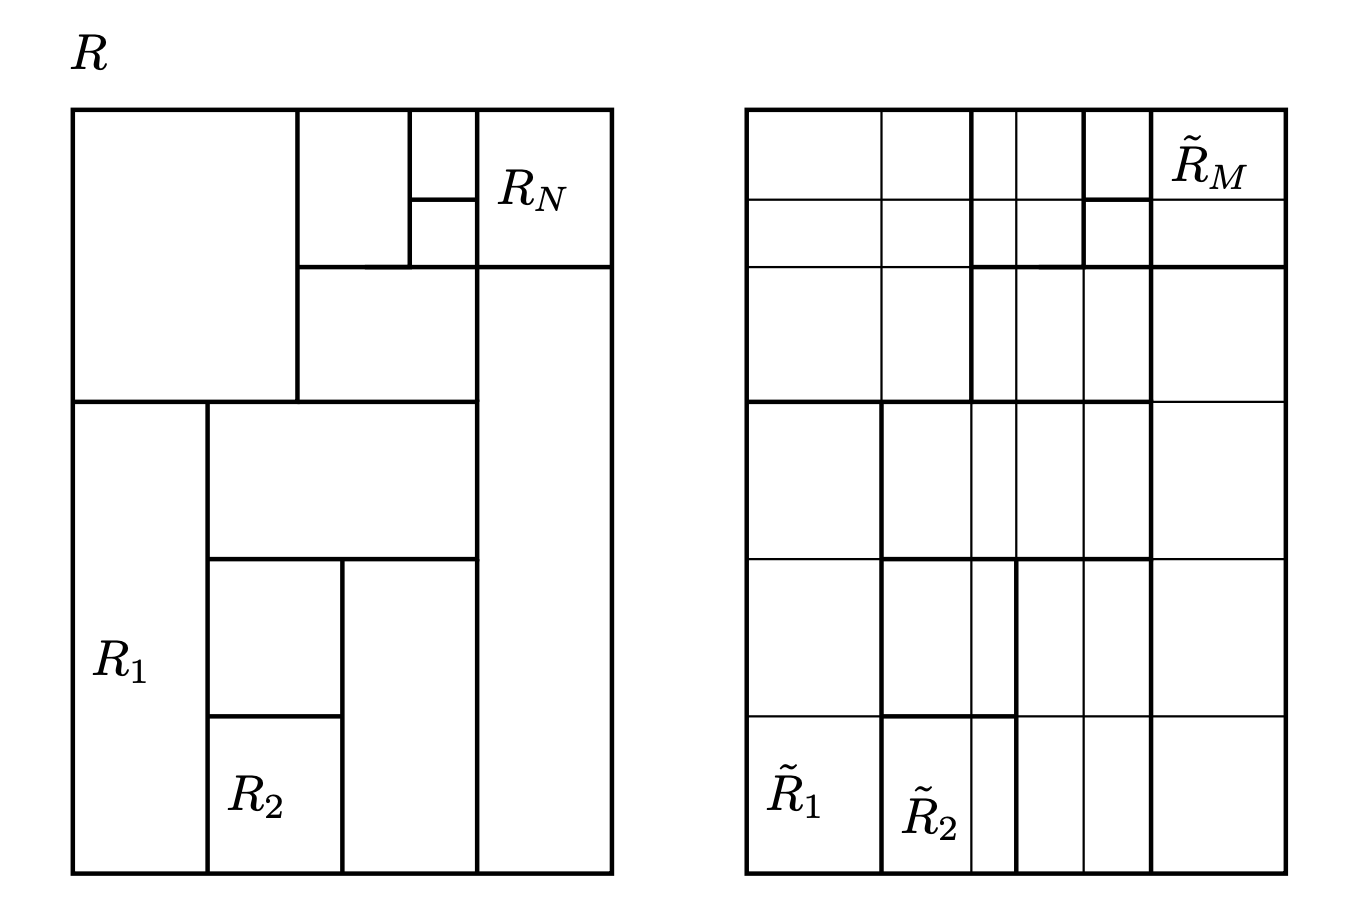
\includegraphics[height=5.5cm]{Figure 1.1.png}
        \caption{The grid formed by the rectangles $R_k$}
    \end{figure}
    For the rectangle $R$, it is clear that $|R|=\sum_{j=1}^{M}{|\tilde{R}_j|}$. By the same reason, we also have $|R_k|=\sum_{j\in J_k}{|\tilde{R}_j|}$. Therefore, one can obtain

    \[|R|=\sum_{j=1}^{M}{|\tilde{R}_j|}=\sum_{k=1}^{N}{\sum_{j\in J_k}{|\tilde{R}_j|}}=\sum_{k=1}^{N}{|R_k|}.\]
\end{proof}
\vspace{5mm}
\begin{tcolorbox}[colback=yellow!10!white,colframe=red!75!black,title=Lemma 1.1.2]\label{Lemma 1.1.2}
    \emph{If $R, R_1,\dots,R_N$ are rectangles, and $R\subseteq\bigcup_{k=1}^{N}{R_k}$, then}
    \[|R|\leq \sum_{k=1}^{N}{|R_k|}.\]
\end{tcolorbox}
\begin{proof}
    As we did in Lemma \hyperref[Lemma 1.1.1]{1.1.1}, we can find smaller rectangles $\tilde{R}_1,\dots,\tilde{R}_M$. Note that there exist $J_0\subseteq\{1,\dots, M\}$ such that $R=\bigcup_{j\in J_0}{\tilde{R}_j}$. Let $R'\coloneqq\bigcup_{j=1}^{M}{\tilde{R}_j}$. Again, we can find a partition $J_1,\dots, J_N$ of $\{1,\dots, M\}$ such that 

    \[R_k=\bigcup_{j\in J_k}{\tilde{R}_j}\quad\text{for all}\quad 1\leq k\leq N.\]
    \\
    Note that $J_0, J_1,\dots, J_N$ need not be disjoint. 
    
    Since $R\subseteq\bigcup_{k=1}^{N}{R_k}$, we have $J_0\subseteq\bigcup_{k=1}^{N}{J_k}$. Therefore, we can obtain

    \[|R|=\sum_{j\in J_0}{|\tilde{R}_j|}\leq \sum_{k=1}^{N}{\sum_{j\in J_k}{|\tilde{R}_j|}}=\sum_{k=1}^{N}{|R_k|}.\]
    \\
    This completes the proof.
\end{proof}
\vspace{5mm}
\begin{tcolorbox}[colback=yellow!10!white,colframe=red!75!black,title=Theorem 1.1.3]\label{Theorem 1.1.3}
    \emph{Every open set $U\subseteq\BR$ can be written uniquely as a countable union of disjoint open intervals.}
\end{tcolorbox}
\begin{proof}
    For each $x\in U$, there exists an open interval, which contains $x$, contained in $U$. If $a_x=\inf\{a<x:(a,x)\subseteq U\}$ and $b_x=\sup\{b>x:(x,b)\subseteq U\}$, then 

    \[x\in I_x\coloneqq(a_x,b_x)\subseteq U.\]
    \\
    Hence, we get $U=\bigcup_{x\in U}{I_x}$. Moreover, note that $I_x$ is the largest open interval, which contains $x$, contained in $U$. 

    Suppose that two intervals $I_x$ and $I_y$ intersect. Then we have

    \[x\in I_x\cup I_y\subseteq U;\]
    \\
    by the maximality of $I_x$, we conclude that $(I_x\cup I_y)\subseteq I_x$. By the same argument, since $(I_x\cup I_y)\subseteq I_y$, we finally have $I_x=I_y$. Therefore, any two distinct intervals in $\mathcal{C}\coloneqq\{I_x\}_{x\in U}$ is disjoint.

    We claim that $\mathcal{C}$ is countable, i.e., it has countably many disjoint open intervals. Since each $I_x$ contains a rational number, any two distinct intervals must contain distinct rationals. Hence, the collection $\mathcal{C}$ must be countable.
\end{proof}
\vspace{5mm}

However, in $\BR^d$ for $d\geq 2$, the direct analogue of Theorem \hyperref[Theorem 1.1.3]{1.1.3} is not valid (see Exercise \hyperref[Exercise 1.12]{1.12}). Instead, there is a substitute result as follows:
\vspace{5mm}
\begin{tcolorbox}[colback=yellow!10!white,colframe=red!75!black,title=Theorem 1.1.4]\label{Theorem 1.1.4}
    \emph{Every open subset $\mathcal{O}\subseteq\BR^d$, $d\geq 1$, can be written as a countable union of almost disjoint closed cubes.}
\end{tcolorbox}
\begin{proof}
    
\end{proof}








\newpage
\section{The exterior measure}

\newpage
\section{Measurable sets and the Lebesgue measure}

\newpage
\section{Measurable functions}

\newpage
\section{Exercises}



\chapter{Integration Theory}
\section{The Lebesgue integral: basic properties and convergence theorems}
\section{The space $L^1$ of integrable functions}
\section{Fubini's theorem}
\section{A Fourier inversion formula}
\section{Exercises}

\chapter{Differentiation and Integration}
\section{Differentiation of the integral}
\section{Good kernels and approximations to the identity}
\section{Differentiability of functions}
\section{Rectifiable curves and the isoperimetric inequality}
\section{Exercises}

\chapter{Solution for exercises}
\begin{center}
    \vspace*{4cm}
        
    \Huge
    \textbf{MAS441: Lebesgue Intergral Theory\\\vspace{2mm}
    Homework Problems}

    \vspace{1cm}
    \large
    Solutions for the selected exercises
    \vspace{3cm}
    
    \LARGE
    \textbf{Jaeho Shin}
        
    \vspace{5cm}
        
    \normalsize
    \textbf{Department of Mathematical Sciences, KAIST}\\  
\end{center}
\newpage
\section{Chapter 1}
\begin{tcolorbox}[colback=yellow!10!white,colframe=gray!75!black,title=Exercise 1.5]\label{Exercise 1.5}
    Suppose $E$ is a given set, and $\mathcal{O}_n$ is the open set:

    \[\mathcal{O}_n=\{x:d(x,E)<1/n\}.\]
    \\
    Show:
    \begin{enumerate}
        \item [(a)] If $E$ is compat, then $m(E)=\lim_{n\rightarrow\infty}{m(\mathcal{O}_n)}$.
        \item [(b)] However, the conclusion in (a) may be false for $E$ closed and unbounded; or $E$ open and bounded.
    \end{enumerate}
\end{tcolorbox}
\begin{proof}
    (a) We first prove that $\mathcal{O}_n$ is open for all $n\in\BZ^+$. For any $x\in\mathcal{O}_n$, since $d(x,E)<\frac{1}{n}$, there exists $\epsilon>0$ such that $d(x,E)+ \epsilon<\frac{1}{n}$. For any $y\in B_d(x,\epsilon)$, by the triangle inequality,

    \begin{align*}
        d(y,E) &= \inf\{d(y,z):z\in E\}\\
        &\leq\inf\{d(y,x)+d(x,z):z\in E\}\\
        &<\epsilon + \inf\{d(x,z):z\in E\}\\
        &=\epsilon+d(x,E)<\frac{1}{n}.
    \end{align*}
    \\
    Therefore, we conclude that $x\in B_d(x,\epsilon)\subseteq\mathcal{O}_n$, that is, $\mathcal{O}_n$ is open.

    Recall that all open sets are measurable and the countable intersection of measurable sets is measurable. Then

    \[\mathcal{O}\coloneqq\bigcap_{n=1}^{\infty}{\mathcal{O}_n}=\{x:d(x,E)=0\}\]
    \\
    is measurable. It is clear that $E\subseteq\mathcal{O}$, by definition. However, since the compactness of $E$ implies that $\bar{E}=E$, note that

    \begin{align*}
        d(x,E)=0\quad&\Longleftrightarrow\quad\forall\epsilon>0,\ \exists y\neq x\ \text{such that}\ y\in E\cap B_d(x,\epsilon)\\
        &\Longleftrightarrow\quad x\in\bar{E}\\
        &\Longleftrightarrow\quad x\in E\quad(\because E\ \text{is compact}.)
    \end{align*}
    \\
    Thus, we get $\mathcal{O}=E$. Moreover, since $\mathcal{O}_n\supseteq\mathcal{O}_{n+1}$, for all $n\in\BZ^+$, we have $\mathcal{O}_n\searrow\mathcal{O}$. 

    One more thing we need to check is whether $m(\mathcal{O}_1)$ is finite or not. Note that the compactness of $E$ implies that it is bounded, i.e., there exists $N>0$ such that $E\subseteq B_d(\mathbf{0},N)$ where $\mathbf{0}$ is the origin. Then, the triangle inequality implies that $\mathcal{O}_1\subseteq B_d(\mathbf{0},N+1)$; therefore, 
    
    \[m(\mathcal{O}_1)\leq m\big(B_d(\mathbf{0},N+1)\big)<\infty.\]
    \\
    Then, by Corollary 1.3.3 in the Textbook, since $\{\mathcal{O}_n\}_{n=1}^{\infty}$ are the measurable sets satisfying $\mathcal{O}_n\searrow E$ and $m(\mathcal{O}_1)<\infty$, we conclude that 

    \[m(E)=\lim_{n\rightarrow\infty}{m(\mathcal{O}_n)}.\]

    \vspace{5mm}
    (b) We fisrt consider the case when $E$ is closed and unbounded. Let $E=\BZ\subseteq\BR$, then it is closed but it is unbounded. Note that

    \[\mathcal{O}_n=\bigcup_{x\in\BZ}{\left(x-\frac{1}{n},x+\frac{1}{n}\right)}\quad\text{for all}\quad n\in\BZ^+.\]
    \\
    Although each interval $(x-1/n,x+1/n)$ has length (or measure) $2/n$, but since there are infinitely many integers, $m(\mathcal{O}_n)$ is infinite for all $n\in\BZ^+$. 
    
    On the other hand, since $\BZ$ is the countable union of singletons, $\{x\}$ with $x\in\BZ$, and since each singleton has measure zero, it follows that $\BZ$ is measurable. Moreover, since these singletons are disjoint measurable sets, we have
    
    \[m(\BZ)=m\left(\bigcup_{x\in\BZ}{\{x\}}\right)=\sum_{x\in\BZ}{m(\{x\})}=0.\]
    \\
    Therefore, we can obtain $m(E)\neq\lim_{n\rightarrow\infty}{m(\mathcal{O}_n)}$, in this case.

    \vspace{5mm}
    Likewise, let's consider the case when $E$ is open and bounded. Since $[0,1]\cap\BQ$ contains countably many elements, let's label them $r_i$ where $i\in\BZ^+$ so that $\{r_1,r_2,\dots\}=[0,1]\cap\BQ$. Under this notation, define 

    \[E\coloneqq\bigcup_{k=1}^{\infty}{\left(r_k-\frac{1}{2^{k+2}},r_k+\frac{1}{2^{k+2}}\right)}\]
    \\
    which is open by being countable union of open intervals. 

    Recall that $\mathcal{O}_n=\{x:d(x,E)<\frac{1}{n}\}$. Hence, we clearly have $\mathcal{O}_n\supseteq\mathcal{O}_{n+1}$ for all $n\in\BZ^+$; moreover, each $\mathcal{O}_n$ is measurable by being an open set. Let

    \[\mathcal{O}\coloneqq\bigcap_{n=1}^{\infty}{\mathcal{O}_n}=\{x:d(x,E)=0\},\]
    \\
    then, as we did before, we have
    
    \begin{align*}
        d(x,E)=0\quad&\Longleftrightarrow\quad\forall\epsilon>0,\ \exists y\neq x\ \text{such that}\ y\in E\cap B_d(x,\epsilon)\\
        &\Longleftrightarrow\quad x\in\bar{E}.
    \end{align*}
    \\
    Hence, we conclude that $\mathcal{O}=\bar{E}$. This implies that $\mathcal{O}_n\searrow\bar{E}$ where $m(\mathcal{O}_1)<\infty$ (since $E$ is bounded, so is $\mathcal{O}_1$); therefore, we get

    \[\lim_{n\rightarrow\infty}{m(\mathcal{O}_n)}=m(\bar{E}).\]
    \\
    Here, since $\bar{E}$ is a well-defined closed set, so it is measurable. Hence, this proves the existence of $\lim_{n\rightarrow\infty}{m(\mathcal{O}_n)}$.
    
    For any $x\in [0,1]$ and $n\geq1$, if $x+\frac{1}{n}\leq 1$, then there exists $m\in\BZ^+$ such that $r_m\in (x,x+\frac{1}{n})$ so that $x\in\mathcal{O}_n$; likewise, if $x+\frac{1}{n}>1$, then there exists $m\in\BZ^+$ such that $r_m\in (x-\frac{1}{n},x)$ so that $x\in\mathcal{O}_n$. Hence, we have $[0,1]\subseteq\mathcal{O}_n$ for all $n\in\BZ^+$. Then the monotonicity gives

    \[1=m\big([0,1]\big)\leq m(\mathcal{O}_n)\quad\text{for all}\quad n\geq1.\]
    \\
    Therefore, we conclude that $\lim_{n\rightarrow\infty}{m(\mathcal{O}_n)}\geq 1$.
    
    However, from the definition of $E$, the countable subadditivity gives that

    \[m(E)\leq\sum_{k=1}^{\infty}{m\left(\Big(r_k-\frac{1}{2^{k+2}},r_k+\frac{1}{2^{k+2}}\Big)\right)}=\sum_{k=1}^{\infty}{\frac{1}{2^{k+1}}}=\frac{1}{2}.\]
    \\
    Hence, we proved that

    \[m(E)\neq\lim_{n\rightarrow\infty}{m(\mathcal{O}_n)}.\]
\end{proof}

\newpage

\begin{tcolorbox}[colback=yellow!10!white,colframe=gray!75!black,title=Exercise 1.8]\label{Exercise 1.8}
    Suppose $L$ is a linear transformation on $\BR^d$. Show that if $E$ is measurable subset of $\BR^d$, then so is $L(E)$, by proceeding as follows:
    \vspace{5mm}
    \begin{enumerate}
        \item [(a)] Note that if $E$ is compact, so is $L(E)$. Hence if $E$ is an $F_\sigma$ set, so is $L(E)$.
        \item [(b)] Because $L$ automatically satisfies the inequality 

        \[|L(x)-L(x')|\leq M|x-x'|\]
        \\
        for some $M$, we can see that $L$ maps any cube of side length $l$ into a cube of side length $c_d Ml$, with $c_d=2\sqrt{d}$. Now if $m(E)=0$, there is a collection of cubes $\{Q_j\}$ such that $E\subset\bigcup_{j}{Q_j}$, and $\sum_{j}{m(Q_j)}<\epsilon$. Thus $m_*{(L(E))}\leq c'\epsilon$, and hence $m(L(E))=0$. Finally, use Corollary 3.5. 
    \end{enumerate}
    \vspace{5mm}
    One can show that $m(L(E))=|\det{L}|m(E)$; see Problem 4 in the next chapter.
\end{tcolorbox}
\begin{proof}
    (a) Since we know that every linear transformation on $\BR^d$ is Lipschitz, thus $L$ is a continuous map. Hence, it maps a compact set $E$ to a compact set, that is, $L(E)$ is compact. 

    Assume that $E$ is an $F_\sigma$ set, i.e. $E=\bigcup_{n=1}^{\infty}{F_n}$ where $\{F_n\}_{n=1}^{\infty}$ are closed sets in $\BR^d$. We now claim that $L(E)$ is also compact. To prove this, we first prove the following lemma:
    \vspace{5mm}
    
    \begin{quote}
        \textbf{Lemma.} Every closed in $\BR^d$ is a countable union of compact sets.
        \begin{proof}
            Let $F$ be a closed set in $\BR^d$. For each $m\in\BZ^+$, let

            \[K_m\coloneqq F\cap\ov{B_d(\mathbf{0},m)}.\]
            \\
            Since $K_m$ is closed and bounded in $\BR^d$, thus it is compact. Also, it is clear that

            \[F=\bigcup_{m=1}^{\infty}{K_m};\]
            \\
            therefore, any closed set $F$ can be written as a countable union of compact sets.
        \end{proof}
    \end{quote}
    \vspace{5mm}
    By lemma, each closed set $F_n$ can be written as 

    \[F_n=\bigcup_{m=1}^{\infty}{K_{n,m}}\]
    \\
    where each $K_{n,m}$ is compact. Thus we get 

    \[E=\bigcup_{n=1}^{\infty}{\bigcup_{m=1}^{\infty}{K_{n,m}}}.\]
    \\
    Then, $L(E)$ can be expressed as 

    \[L(E)=\bigcup_{n=1}^{\infty}{\bigcup_{m=1}^{\infty}{L(K_{n,m})}}\]
    \\
    where each $L(K_{n,m})$ is compact, by the above conclusion. Therefore, this implies that $L(E)$ is a countable union of compact sets (which are closed in $\BR^d$) so that it is a $F_\sigma$ set.

    \vspace{5mm}
    (b) If $m(E)=0$, then there exist a collection of closed cubes $\{Q_j\}_{j=1}^{\infty}$ such that 

    \[E\subseteq\bigcup_{j=1}^{\infty}{Q_j}\quad\text{and}\quad 0\leq\sum_{j=1}^{\infty}{|Q_j|}<\epsilon.\]
    \\
    Let $l_j$ be the side length of $Q_j$, for each $j$, then $L(Q_j)$ is contained in a cube $Q_j'$ of side length $c_dMl_j$ where $c_d=2\sqrt{d}$. Since

    \[L(E)\subseteq\bigcup_{j=1}^{\infty}{L(Q_j)}\subseteq\bigcup_{j=1}^{\infty}{Q_j'}\]
    thus 
    \[m_*(L(E))\leq\sum_{j=1}^{\infty}{|Q_j'|}=(c_dM)^d\sum_{j=1}^{\infty}{l_j^d}<\epsilon(c_dM)^d.\]
    \\
    This proves that $m_*(L(E))=0$. 

    Note that since $E$ is measurable, by Corollary 1.3.5, there exist an $F_\sigma$ set $F$ such that 
    
    \[m(E\triangle F)=0.\]
    \\
    Then, by part (a), $L(F)$ is also $F_\sigma$ set and since we have

    \[L(E)\triangle L(F)\subseteq L(E\triangle F),\]
    \\
    in general, thus 

    \[0\leq m_*\big(L(E)\triangle L(F)\big)\leq m_*\big(L(E\triangle F)\big).\]
    \\
    Since $m(E\triangle F)=0$ implies that $m_*\big(L(E\triangle F)\big)=0$, we get 

    \[m_*\big(L(E)\triangle L(F)\big)=0.\]
    \\
    This implies that $L(E)$ differs from an $F_\sigma$ set $L(F)$ by a set of measure zero; therefore, $L(E)$ is measurable and we conclude that $m(L(E))=0$.
\end{proof}

\newpage

\begin{tcolorbox}[colback=yellow!10!white,colframe=gray!75!black,title=Exercise 1.11]\label{Exercise 1.11}
    Let $A$ be the subset of $[0,1]$ which consists of all numbers which do not have the digit 4 appearing in their decimal expansion. Find $m(A)$.
\end{tcolorbox}

\begin{proof}
    Let $A_n$ denote the set 

    \[A_n\coloneqq\{x\in [0,1]:\text{first $n$ digits of $x$ do not contain 4}\}.\]
    \\
    for all $n\in\BZ^+$. Then $A_{n+1}\subseteq A_n$, for all $n$, and 

    \[A=\bigcap_{n=1}^{\infty}{A_n}.\]
    \\
    This implies that $A_n\searrow A$.

    Note that each $A_n$ is a finite union of intervals. For instance, since $A_1$ is 

    \[A_1=\left[0,\frac{4}{10}\right)\cup\left[\frac{5}{10},1\right],\]
    \\
    thus it is measurable and has measure $9/10$. Similarly, $A_2$ is obtained from $A_1$ by removing 9 subintervals of length $1/100$, corresponding to numbers whose second digit is 4. Therefore, we get $m(A_2)=\left(9/10\right)^2$. By repeating this procedure, we have
    
    \[m(A_n)=\left(\frac{9}{10}\right)^n\quad\text{for all}\quad n\in\BZ^+.\]
    \\
    By Corollary 1.3.3, since $\{A_n\}_{n=1}^{\infty}$ are measurable sets with $A_n\searrow A$ and $m(A_1)<\infty$, thus we have
    
    \[m(A)=\lim_{n\rightarrow\infty}{m(A_n)}=\lim_{n\rightarrow\infty}{\left(\frac{9}{10}\right)^n}=0.\]
\end{proof}

\newpage

\begin{tcolorbox}[colback=yellow!10!white,colframe=gray!75!black,title=Exercise 1.12]\label{Exercise 1.12} 
    Theorem 1.3 states that every open set in $\BR$ is the disjoint of open intervals. The analogue in $\BR^d$, $d\geq 2$, is generally false. Prove the following:
    \begin{enumerate}
        \item [(a)] An open disc in $\BR^2$ is not the disjoint union of open rectangles.
        
        [Hint: What happens to the boundary of any of these rectangles?]
        \item [(b)] An open connected set $\Omega$ is the disjoint union of open rectangles if and only if $\Omega$ is itself an open rectangle.
    \end{enumerate}
\end{tcolorbox}
\begin{proof}
    (a) Suppose not. Let $\mathcal{C}$ be the collection of disjoint open rectangles whose union is an open disc in $\BR^2$. Consider $R\in\mathcal{C}$ and $x\in\mathrm{bd}(R)$ which does not lie on the boundary of disc. Since $x\in D$, where $D$ denotes the disc, there exist $R'\in\mathcal{C}$ such that $x\in R'$. Hence, there exist a basis element $B$ (which is an $\epsilon$-ball centered at $x$) such that

    \[x\in B\subseteq R'.\]
    \\
    Since $x\in\mathrm{bd}(R)=\ov{R}\cap\ov{(\BR^d\setminus R)}$ and $B$ is a neighborhood of $x$, so $B$ intersects $R$ at some point $y$ other than $x$. Since $y\in B\subseteq R'$ and $y\in R$, we have $R\cap R'=\emptyset$ which is a contradiction. Therefore, $D$ cannot be the disjoint union of open rectangles.

    \vspace{5mm}
    (b) Suppose that $\Omega=\bigcup_{U\in\mathcal{C}}{U}$ where the elements of $\mathcal{C}$ are disjoint open rectangles. Let $\emptyset\neq\mathcal{A}\subsetneq\mathcal{C}$. Then 

    \[\Omega=\left(\bigcup_{U\in\mathcal{A}}{U}\right)\cup\left(\bigcup_{U\in\mathcal{C}\setminus\mathcal{A}}{U}\right)\]
    \\
    gives a separation of $\Omega$ which contradicts to the connectedness of $\Omega$. Therefore, such $\mathcal{A}$ cannot exist, i.e., $|\mathcal{C}|=1$ so that $\Omega$ is an open rectangle.
    The converse is trivial; hence, the proof is done.
\end{proof}

\newpage

\begin{tcolorbox}[colback=yellow!10!white,colframe=gray!75!black,title=Exercise 1.16]\label{Exercise 1.16}
    Suppose $\{E_k\}_{k=1}^{\infty}$ is a countable family of measurable subsets of $\BR^d$ and that

    \[\sum_{k=1}^{\infty}{m(E_k)}<\infty.\]
    \\
    Let 
    \begin{align*}
        E &= \{x\in\BR^d: x\in E_k,\ \text{for infinitely many $k$}\}\\
        &= \limsup_{k\rightarrow\infty}{(E_k)}.
    \end{align*}
    \begin{enumerate}
        \item [(a)] Show that $E$ is measurable.
        \item [(b)] Prove $m(E)=0$.
    \end{enumerate}
    [Hint: Write $E=\bigcap_{n=1}^{\infty}{\bigcup_{k\geq n}{E_k}}$.]
\end{tcolorbox}
\begin{proof}
    (a) Recall that $\limsup_{k\rightarrow\infty}(E_k)$ is obtained by

    \[\limsup_{k\rightarrow\infty}(E_k)=\bigcap_{n=1}^{\infty}{\bigcup_{k=n}^{\infty}{E_k}}.\]
    \\
    This is because 
    \begin{align*}
        \text{$x\in E_k$ for infinitely many $k$}\quad&\Longleftrightarrow\quad x\in\bigcup_{k=n}^{\infty}{E_k}\ \text{for all $n\in\BZ^+$}\\
        &\Longleftrightarrow\quad x\in\bigcap_{n=1}^{\infty}{\bigcup_{k=n}^{\infty}{E_k}}.
    \end{align*}
    \\
    Since each $E_k$ is measurable, so is $\bigcup_{k=n}^{\infty}{E_k}$. Likewise, this implies that $\bigcap_{n=1}^{\infty}{\bigcup_{k=n}^{\infty}{E_k}}$ is also measurable. Therefore, we conclude that $E$ is measurable.

    \vspace{5mm}
    (b) $\sum_{k=1}^{\infty}{m(E_k)}<\infty$ implies that, for any $\epsilon>0$, there exists $N>0$ such that
    
    \[\sum_{k=N}^{\infty}{m(E_k)}<\epsilon.\]
    \\
    Then, by the countable subadditivity, we have

    \[m\left(\bigcup_{k=N}^{\infty}{E_k}\right)\leq\sum_{k=N}^{\infty}{m(E_k)}<\epsilon.\]
    \\
    However, since the monotonicity implies that

    \[m(E)=m\left(\bigcap_{n=1}^{\infty}{\bigcup_{k=n}^{\infty}{E_k}}\right)\leq m\left(\bigcup_{k=N}^{\infty}{E_k}\right)<\epsilon,\]
    \\
    we conclude that $m(E)=0$.
\end{proof}

\newpage

\begin{tcolorbox}[colback=yellow!10!white,colframe=gray!75!black,title=Exercise 1.17]\label{Exercise 1.17}
    Let $\{f_n\}$ be a sequence of measurable functions on $[0,1]$ with $|f_n(x)|<\infty$ for a.e $x$. Show that there exists a sequence $c_n$ of positive real numbers such that

    \[\frac{f_n(x)}{c_n}\rightarrow 0\quad\text{a.e.}\quad x\]

    \vspace{5mm}
    \noindent[Hint: Pick $c_n$ such that $m(\{x:|f_n(x)/c_n|>1/n\})<2^{-n}$, and apply the Borel-Cantelli lemma.]
\end{tcolorbox}
\begin{proof}
    The fact that $|f_n(x)|<\infty$ for a.e $x$ implies that 

    \[m\big(\{x:|f_n(x)|=\infty\}\big)=0.\]
    \\
    Let $A$ denote the set $\{x:|f(x)|=\infty\}$. If we let $A_k\coloneqq\{x:|f_n(x)|>k/n\}$ for all $k\in\BZ^+$, then we have $A_k\searrow A$ since 

    \[A_{k+1}\subseteq A_k\quad\text{for all}\quad k\in\BZ^+\]
    and
    \[\bigcap_{k=1}^{\infty}{A_k}=\{x:|f_n(x)|=\infty\}.\]
    \\
    Therefore, we get 

    \[\lim_{k\rightarrow\infty}{m(A_k)}=m(A)=0.\]
    \\
    This implies that there exists $c_n\in\BZ^+$ such that $m(A_{c_n})<2^{-n}$, i.e.

    \[m\left(\left\{x:|f_n(x)|>\frac{c_n}{n}\right\}\right)<2^{-n}.\tag{\(*\)}\]
    \\
    Define, for all $n\in\BZ^+$, 

    \[E_n=\left\{x:\left|\frac{f_n(x)}{c_n}\right|>\frac{1}{n}\right\}.\]
    \\
    Then $(*)$ implies that $m(E_n)<2^{-n}$ for all $n$. Note that $\{E_n\}_{n=1}^{\infty}$ is a countable family of measurable sets with

    \[\sum_{n=1}^{\infty}{m(E_n)}<\sum_{n=1}^{\infty}{\frac{1}{2^n}}=1<\infty;\]
    \\
    therefore, by the Borel-Cantelli lemma, we get $m(E)=0$ where

    \[E\coloneqq\limsup_{n\rightarrow\infty}{(E_n)}.\]
    \\
    For any $x\in E^c$, there exists $N>0$ such that $x\notin E_n$ for all $n\geq N$. This implies that

    \[\lim_{n\rightarrow\infty}{\left|\frac{f_n(x)}{c_n}\right|}=0\quad\text{for all}\quad x\in E^c.\]
    \\
    Therefore, $m(E)=0$ implies that     

    \[\frac{f_n(x)}{c_n}\rightarrow0\quad\text{a.e.}\quad x.\]
\end{proof}

\newpage

\begin{tcolorbox}[colback=yellow!10!white,colframe=gray!75!black,title=Exercise 1.20]\label{Exercise 1.20.}
    Show that there exist closed sets $A$ and $B$ with $m(A)=m(B)=0$, but $m(A+B)>0$:
    \begin{enumerate}
        \item [(a)] In $\BR$, let $A=\mathcal{C}$ (the Cantor set), $B=\mathcal{C}/2$. Note that $A+B\supset [0,1]$.
        \item [(b)] In $\BR^2$, observe that if $A=I\times\{0\}$ and $B=\{0\}\times I$ (where $I=[0,1]$), then $A+B=I\times I$.
    \end{enumerate}
\end{tcolorbox}
\begin{proof}
    (a) It is clear that every number in $[0,1]$ has a ternary expansion 

    \[x=\sum_{k=1}^{\infty}{a_k3^{-k}},\quad\text{where}\quad a_k=0,1, \text{or}\ 2.\]
    \\
    The algorithm for finding $a_k$ is as following: If $x=1$, then $a_k=2$ for all $k\in\BZ^+$; if $x<1$, take $a_1=\lfloor 3x\rfloor$ where $\lfloor\cdot\rfloor$ denotes the greatest integer less than or equal to $x$. Similarly, we take $a_2=\lfloor3(3x-a_1)\rfloor$ and by repeating this procedure, we have

    \[a_n=\left\lfloor3^nx-\sum_{k=1}^{n-1}{a_k3^{n-k}}\right\rfloor\quad\text{for all}\quad n\geq 2.\]
    \\
    Note that the ternary expansion is not unique since, for example, $1/3=\sum_{k=2}^{\infty}{2/3^k}$.

    Since $A=\mathcal{C}$, the Cantor set, $A$ consists of all numbers which have a ternary expansion with $a_k\in\{0,2\}$ for all $k\in\BZ^+$. By the same reason, since $B=\mathcal{C}$, it consists of all numbers which have a ternary expansion with $a_k\in\{0,1\}$.

    Now we claim that, for any $x\in [0,1]$, there exist $a\in A$ and $b\in B$ such that $x=a+b$. Let $x=\sum_{k=1}^{\infty}{a_k3^{-k}}$, where $a_k\in\{0,1,2\}$, be a ternary expansion of $x$. Likewise, let

    \[a=\sum_{k=1}^{\infty}{a_k3^{-k}}\quad\text{and}\quad b=\sum_{k=1}^{\infty}{b_k3^{-k}}\]
    \\
    be ternary expansions of $a$ and $b$, respectively. By letting, 

    \[a_k=\begin{cases}
        2, & \text{if $x_k=2$}\\
        0, & \text{otherwise}
    \end{cases}\quad\text{and}\quad b_k=\begin{cases}
        1, & \text{if $x_k=1$}\\
        0, & \text{otherwise}
    \end{cases}\]
    \\
    we clearly have $x=a+b$ (since $x_k=a_k+b_k$ for all $k\in\BZ^+$). Therefore,

    \[[0,1]\subseteq A+B.\]

    \vspace{5mm}
    (b) Let $x=(x_1,x_2)\in A+B$, then $x=a+b$ for some $a\in A$ and $b\in B$. Since $a$ and $b$ are of the form $a=(a',0)$ and $b=(0,b')$ where $a',b'\in I$. Then

    \[(x_1,x_2)=(a',0)+(0,b')\quad\Longrightarrow\quad x_1=a'\quad\text{and}\quad x_2=b';\]
    \\
    therefore, $(x_1,x_2)\in I\times I$. 

    Conversely, assume that $x=(x_1,x_2)\in I\times I$. Since each $x_1$ and $x_2$ belongs to $I$, it is clear that $(x_1,0)\in A$, $(0,x_2)\in B$, and

    \[x=(x_1,0)+(0,x_2)\in A+B.\]
    \\
    Therefore, we get $I\times I\subseteq A+B$ and this completes the proof.

    \vspace{5mm}
    \emph{In part (a), note that both $A$ and $B$ are closed with measure zero, but $A+B$ has positive measure since $A+B\supset [0,1]$. Likewise, note that $A$ and $B$ in part (b) are also closed with measure zero, but $A+B=I\times I$ has positive measure, obviously.}
\end{proof}

\newpage

\begin{tcolorbox}[colback=yellow!10!white,colframe=gray!75!black,title=Exercise 1.21]\label{Exercise 1.21} 
    Prove that there is a continuous function that maps a Lebesgue measurable set to a non-measurable set.

    \noindent [Hint: Consider a non-measurable subset of $[0,1]$, and its inverse image in $\mathcal{C}$ by the function $F$ in Exercise 2.]
\end{tcolorbox}
\begin{proof}
    Let $\mathcal{C}$ denote the Cantor set. Define a map $f:\mathcal{C}\rightarrow [0,1]$ to because
    
    \[f(x)=\sum_{k=1}^{\infty}{\frac{b_k}{2^k}}\qquad\text{if}\ x=\sum_{k=1}^{\infty}{a_k3^{-k}},\ \text{where}\ b_k=a_k/2.\]
    \\
    In this definition, we choose the expansion of $x$ in which $a_k=0\ \text{or}\ 2$. We first claim that $f$ is well-defined and continuous on $\mathcal{C}$, and moreover it is surjective.
    \vspace{5mm}
    \begin{enumerate}
        \item []\textbf{(Well-definedness).} Since we proved that every number in $[0,1]$ has at least one ternary expansion, the only problem is that some numbers (such as $1/3$) have more than one ternary expansions. However, such a number can have a unique ternary expansion that consists of all 0's and 2's, because the only problem arises when one representation terminates while the other doesn't. If a representation terminates, then it must end with $2$ (if it contains only 0's and 2's). However, then the other expansion ends with $1222\cdots$; therefore, it contains 1 in its expansion. This proves that each element of $\mathcal{C}$ has the unique ternary expansion consists of only 0's and 2's; hence, the map $f$ is well-defined.
        \item []
        \item []\textbf{(Continuity).} For any $\epsilon>0$, there exists $n\in\BZ^+$ such that $1/2^n<\epsilon$. Let $\delta=1/3^n$, then for any $x,y\in\mathcal{C}$ with $|x-y|<\delta$, first $n$ digits of their ternary expansion must be the same. Otherwise, one must contain 1 in its expansion or their difference must be greater than or equal to $\delta$. Therefore, for such $x$ and $y$, we have
        
        \[|f(x)-f(y)|<\sum_{k=n+1}^{\infty}{\frac{1}{2^k}}=\frac{1}{2^n}<\epsilon.\]
        \\
        Therefore, we conclude that $f$ is continuous.
        \item []
        \item []\textbf{(Surjectivity).} As we did in Exercise 1.20, every number in $[0,1]$ also has a binary expansion
        
        \[x=\sum_{k=1}^{\infty}{b_k2^{-k}},\quad\text{where}\quad b_k=0\ \text{or}\ 1.\]
        \\
        If $x<1$, then $b_k=1$ for all $k\in\BZ^+$; if $x<1$, then $b_1=\lfloor 2x\rfloor$ and 

        \[b_n=\left\lfloor2^nx-\sum_{k=1}^{n-1}{a_k2^{n-k}}\right\rfloor\quad\text{for all}\quad n\geq 2.\]
        \\
        Hence, for any $y\in [0,1]$, it has a binary expression

        \[y=\sum_{k=1}^{\infty}{b_k2^{-k}}.\]
        \\
        Let $a_k\coloneqq 2b_k$ for all $k\in\BZ^+$. Since $a_k$ if either 0 or 2, for all $k$, 
        
        \[x\coloneqq\sum_{k=1}^{\infty}{a_k3^{-k}}\]
        \\
        belongs to $\mathcal{C}$. Moreover, it is clear that $f(x)=y$; therefore, $f$ is surjective.
    \end{enumerate}
    \vspace{5mm}

    Note that the set $\mathcal{N}$ defined in the Theorem 1.3.6 is non-measurable subset of $[0,1]$. Let $E\coloneqq f^{-1}(\mathcal{N})\subseteq\mathcal{C}$. Since $E$ is a subset of the measure zero set $\mathcal{C}$, we have $m(E)=0$. This implies that $E$ is measurable. Therefore, $f$ is a continuous function which maps the Lebesgue measurable set $E$ to a non-measurable set $\mathcal{N}$.
\end{proof}

\newpage

\begin{tcolorbox}[colback=yellow!10!white,colframe=gray!75!black,title=Exercise 1.22]\label{Exercise 1.22}
    Let $\chi_{[0,1]}$ be the characteristic function of $[0,1]$. Show that there is no everywhere continuous function $f$ on $\BR$ such that 

    \[f(x)=\chi_{[0,1]}(x)\quad\text{almost everywhere}.\]
\end{tcolorbox}
\begin{proof}
    Suppose that such a continuous function $f$ exists. We first claim that 
    
    \[f(x)=0\quad\text{for all}\quad x\in(-\infty,0).\]
    \\
    Assume that there exists $x_0\in(-\infty,0)$ such that $f(x_0)\neq 0$. Then, since $f$ is continuous, for any $0<\epsilon<|f(x_0)|$, there exists $\delta>0$ such that

    \[|x-x_0|<\delta\quad\Longrightarrow\quad |f(x)-f(x_0)|<\epsilon.\]
    \\
    Then, for any $x\in (x_0-\delta,x_0]$, the triangle inequality implies that 

    \[|f(x)|\geq|f(x_0)|-|f(x)-f(x_0)|>|f(x_0)|-\epsilon>0.\]
    \\
    Thus, $(x_0-\delta,x_0]\subseteq\{x:f(x)\neq\chi_{[0,1]}(x)\}$ so that

    \[m\left(\{x:f(x)\neq\chi_{[0,1]}(x)\}\right)\geq\delta>0\]
    \\
    which is a contradiction. Therefore, we have $f|_{(-\infty,0)}=0$.

    By the same argument, we can check that $f|_{(0,1)}=1$. If there exists $x_0\in (0,1)$ such that $f(x_0)\neq 1$, then for any $0<\epsilon<|f(x_0)-1|$, there exists $\delta>0$ such that 
    
    \[B_d(x_0,\delta)\subseteq (0,1)\qquad\text{and}\qquad |f(x)-f(x_0)|<\epsilon\quad\text{for all}\quad x\in B_d(x_0,\delta).\] 
    \\
    Therefore, for any $x\in B_d(x_0,\delta)$, the triangle inequality gives 

    \[|f(x)-1|\geq |f(x_0)-1|-|f(x)-f(x_0)|>|f(x_0)-1|-\epsilon>0.\]
    \\
    Thus, $B_d(x_0,\delta)\subseteq\{x:f(x)\neq\chi_{[0,1]}(x)\}$ so that

    \[m\left(\{x:f(x)\neq\chi_{[0,1]}(x)\}\right)\geq2\delta>0\]
    \\
    which is again a contradiction. Therefore, we conclude that $f|_{(0,1)}=1$.

    However, since $f|_{(-\infty,0)}=0$ and $f|_{(0,1)}=1$, it follows that $f$ cannot be continuous at $0$, no matter what value is assigned to $f(0)$. This contradicts to the assumption that $f$ is a continuous function on $\BR$. Therefore, we conclude that there is no everywhere continuous function $f$ on $\BR$ such that $f(x)=\chi_{[0,1]}(x)$ almost everywhere.
\end{proof}

\newpage

\begin{tcolorbox}[colback=yellow!10!white,colframe=gray!75!black,title=Exercise 1.26]\label{Exercise 1.26}
    Suppose $A\subset E\subset B$, where $A$ and $B$ are measurable sets of finite measure. Prove that if $m(A)=m(B)$, then $E$ is measurable.
\end{tcolorbox}
\begin{proof}
    Since $A$ and $B$ are measurable, so is $B\setminus A$. Note that $A$ and $B\setminus A$ are disjoint measurable sets. Therefore, we have

    \[m(B)=m\big(A\cup(B\setminus A)\big)=m(A)+m(B\setminus A),\]
    \\
    and since $m(A)=m(B)$, we get $m(B\setminus A)=0$. 

    Note that $E\setminus A\subseteq B\setminus A$, thus we have

    \[m_*(E\setminus A)\leq m_*(B\setminus A)=0.\]
    \\
    Since $m_*(E\setminus A)=0$, it is measurable. Then, since $E=A\cup (E\setminus A)$ is a union of two measurable set, thus we conclude that $E$ is also measurable.
\end{proof}

\newpage

\begin{tcolorbox}[colback=yellow!10!white,colframe=gray!75!black,title=Exercise 1.28]\label{Exercise 1.28}
    Let $E$ be a subset of $\BR$ with $m_*(E)>0$. Prove that for each $0<\alpha<1$, there exists an open interval $I$ so that

    \[m_*(E\cap I)\geq \alpha m_*(I).\]
    \\
    Loosely speaking, this estimate shows that $E$ contains almost a whole interval.

    \noindent [Hint: Choose an open set $\mathcal{O}$ that contains $E$, and such that $m_*(E)\geq \alpha m_*(\mathcal{O})$. Write $\mathcal{O}$ as the countable union of disjoint open intervals, and show that one of these intervals must satisfy the desired property.]
\end{tcolorbox}
\begin{proof} 
    For any $0<\alpha<1$, let $\mathcal{O}$ be an open set containing $E$ such that $m_*(E)\geq\alpha m_*(\mathcal{O})$. Note that $\mathcal{O}$ can be written as a countable union of disjoint open intervals so that

    \[E=\bigcup_{k=1}^{\infty}{I_k}\]
    \\
    where $\{I_k\}_{k=1}^{\infty}$ are disjoint open intervals. Then we have

    \[E=E\cap\mathcal{O}=\bigcup_{k=1}^{\infty}{(E\cap I_k)};\]
    \\
    hence, by the countable subadditivity, 

    \[m_*(E)\leq\sum_{k=1}^{\infty}{m_*(E\cap I_k)}.\]
    \\
    If there is no open interval $I$ satisfying $m_*(E\cap I)\geq\alpha m_*(I)$, since $\{I_k\}_{k=1}^{\infty}$ are disjoint open sets, we have

    \[m_*(E)<\alpha\sum_{k=1}^{\infty}{m_*(I_k)}=\alpha m_*(\mathcal{O})\leq m_*(E)\]
    \\
    which is a contradiction. Therefore, there exist $k\in\BZ^+$ such that

    \[m_*(E\cap I_k)\geq\alpha m_*(I_k)\]
    \\
    where $I_k$ is an open interval in $\BR$.
\end{proof}

\newpage

\begin{tcolorbox}[colback=yellow!10!white,colframe=gray!75!black,title=Exercise 1.30]\label{Exercise 1.30}
    If $E$ and $F$ are measurable, and $m(E)>0,\ m(F)>0$, prove that 

    \[E+F=\{x+y:x\in E,\ y\in F\}\]
    \\
    contains an interval.
\end{tcolorbox}
\begin{proof}
    Note that $-F=\{-x:x\in F\}$ is also measurable with $m(-F)>0$ since $F$ is measurable. By the Exercise 1.28, for any $0<\alpha<1$, there exist open intervals $I_1$ and $I_2$ such that 

    \[m(E\cap I_1)\geq\alpha m(I_1)\quad\text{and}\quad m(-F\cap I_2)\geq\alpha m(I_2).\]
    \\
    Without loss of generality, assume that $m(I_2)\leq m(I_1)$. Then, since they are intervals, there exists $h\in\BR$ such that $I_2+h\subseteq I_1$. (Here, note that $I_2+h\coloneqq\{x+h:x\in I_2\}$.) For convenience, let $l=m(I_2)>0$. Then, for any $0<|r|<l$, we have 

    \[m\big(I_1\cap (I_2+h+r)\big)\geq l-|r|>0.\]
    \\
    This implies that 

    \[I_1\cap (I_2+h+r)\neq\emptyset;\]
    \\
    hence, there exist $e\in E$, $f\in F$ such that 

    \[e=-f+h+r.\]
    \\
    In other words, for any $0<|r|<l$, 

    \[h+r=e+f\]
    \\
    for some $e\in E$ and $f\in F$. Therefore, we conclude that
    
    \[(h-l,h+l)\subseteq E+F,\]
    \\
    that is, $E+F$ contains an interval.
\end{proof}

\newpage

\begin{tcolorbox}[colback=yellow!10!white,colframe=gray!75!black,title=Exercise 1.37]\label{Exercise 1.37}
    Suppose $\Gamma$ is a curve $y=f(x)$ in $\BR^2$, where $f$ is continuous. Show that $m(\Gamma)=0$. 

    \noindent [Hint: Cover $\Gamma$ by rectangles, using the uniform continuity of $f$.]
\end{tcolorbox}
\begin{proof}
    For each $n\in\BZ$, define 
    
    \[\Gamma_n\coloneqq\{(x,f(x)): x\in[n,n+1]\}\subseteq\BR^2.\]
    \\
    Since $f$ is continuous and $[n,n+1]$ is compact, thus $f$ is uniformly continuous on $[n,n+1]$. This implies that, for any $\epsilon>0$, there exists $\delta>0$ such that

    \[|x-y|<\delta\quad\Longrightarrow\quad |f(x)-f(y)|<\epsilon.\]
    \\
    Note that there exists $N\in\BZ^+$ such that $1/N<\delta$. Let 

    \[I_i\coloneqq\left[n+\frac{i-1}{N},n+\frac{i}{N}\right]\]
    \\
    for each $1\leq i\leq N$. Since, for any $x,y\in I_i$, we have $|f(x)-f(y)|<\epsilon$; thus 

    \[f(x)\in\left[f\left(n+\frac{i-1}{N}\right)-\epsilon,\ f\left(n+\frac{i-1}{N}\right)+\epsilon\right]\]
    \\
    for all $x\in I_i$. Let

    \[R_i\coloneqq \left[f\left(n+\frac{i-1}{N}\right)-\epsilon,\ f\left(n+\frac{i-1}{N}\right)+\epsilon\right]\times I_i\]
    \\
    for each $1\leq i\leq N$. Then, we have

    \[\Gamma_n\subseteq\bigcup_{i=1}^{N}{R_i}\quad\Longrightarrow\quad m_*(\Gamma_n)\leq\sum_{i=1}^{N}{m_*(R_i)}=N\left(2\epsilon\cdot\frac{1}{N}\right)=2\epsilon.\]
    \\
    Since $\epsilon>0$ is chosen arbitrarily, we have $m_*(\Gamma_n)=0$, that is, $\Gamma_n$ is measurable and $m(\Gamma_n)=0$. Finally, since we have

    \[\Gamma=\bigcup_{n\in\BZ^+}{\Gamma_n},\]
    \\
    $\Gamma$ is measurable and by countable subadditivity, we get 

    \[m(\Gamma)\leq\sum_{n\in\BZ}{m(\Gamma_n)}=0\]
\end{proof}

\newpage
\section{Section 2}






\end{document}